\ylDisplay{Lüliti} % Ülesande nimi
{Tundmatu autor} % Autor
{piirkonnavoor} % Voor
{2012} % Aasta
{P 3} % Ülesande nr.
{1} % Raskustase
{
% Teema: Elektriõpetus
\ifStatement
Juku tahab ehitada seadet, mis elektrimootori jõul kardinaid akna ette või eest ära tõmbaks. Selleks võttis ta elektrimootori, lüliti ja suure patarei. Kasutatud lüliti võib olla kolmes asendis ja sellel on 6 klemmi. Lambi ja patareiga katsetades sai Juku teada, et erinevates asendites (A, B või C) ühendab lüliti klemme kokku joonisel kujutatud viisil. Mootor muudab suunda, kui temaga ühendatud patarei klemmid ära vahetada. Kuidas peaks ühendama lüliti, patarei ja mootori, et lüliti erinevate asendite korral pöörleks mootor ühtepidi, teistpidi või oleks  paigal? Joonistage kaks elektriskeemi, kus on lülitit erinevalt kasutatud.
\begin{center}
	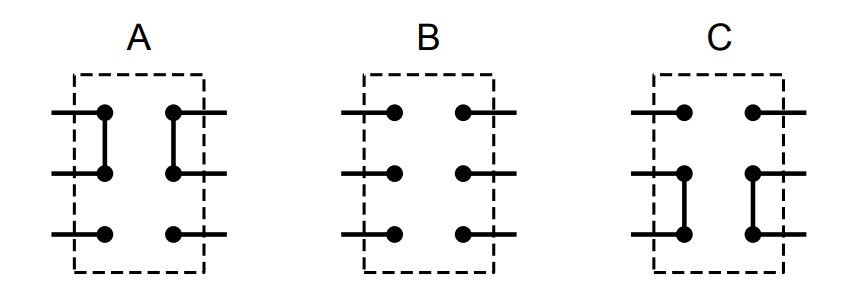
\includegraphics[width=0.5\linewidth]{2012-v2p-03-yl.png}
\end{center}
\fi

\ifHint
Toide on vaja lüliti plokile ühendada nii, et ühes asendis on plussklemm ühendatud mootori parema poolega ja miinusklemm vasaku poolega, et mootor töötaks ühtepidi, kuid teises asendis on pluss- ja miinusklemm ühendatud vastupidi, et mootor töötaks samuti vastassuunas.
\fi

\ifSolution
Võimalikud ühendamisviisid on toodud joonisel.
\begin{center}
	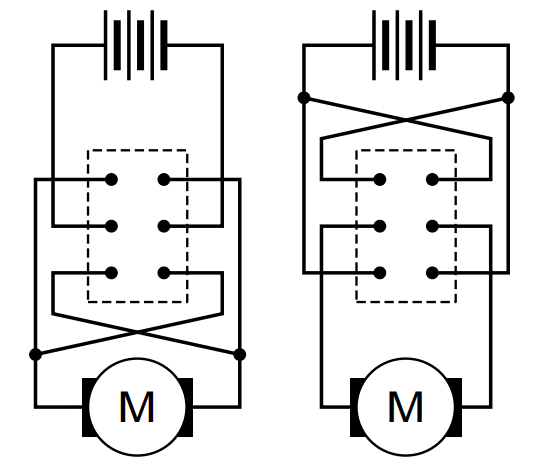
\includegraphics[width=0.5\linewidth]{2012-v2p-03-lah.png}
\end{center}
\fi

}